% !TEX root = ../../prj4projektrapport.tex
% SKAL STÅ I TOPPEN AF ALLE FILER FOR AT MASTER-filen KOMPILERES 

\section{Design og implementering}
I dette afsnit beskrives, hvordan Måleenheden er udviklet. Måleenheden er designet til at kunne måle strøm og spænding centralt og decentralt. Spændingen måles direkte mellem fase og nul, hvor strømmen måles, ved at måle spænding hen over en 1$\Omega$ modstand i serie med hver forbruger og transmissionslinje. 

\subsection{Hardware}
PSOC'ens sample område ligger mellem 0 og 5V, hvor signalerne til spændingen og strømmen forventes at svinge omkring 0V. Derfor er der udviklet hardware der kan hæve signalerne til at svinge omkring 2,5V. Måleenheden skal kunne måle op til 8V, så derfor har det været nødvendigt at dæmpe spændings signalet. Strøm niveauet er tilgengæld meget lille, hvor vi derfor gerne vil forstærke det. På figurer \ref{fig:MaalHardware} ses diagrammet for hardwaren. Det er valgt at bruge operations forstærkeren AD823, da den kan forsynes med 5Vdc og udnytte hele dens forsyningsspændings område.  

\begin{figure}[htbp] % (alternativt [H])
	\centering
	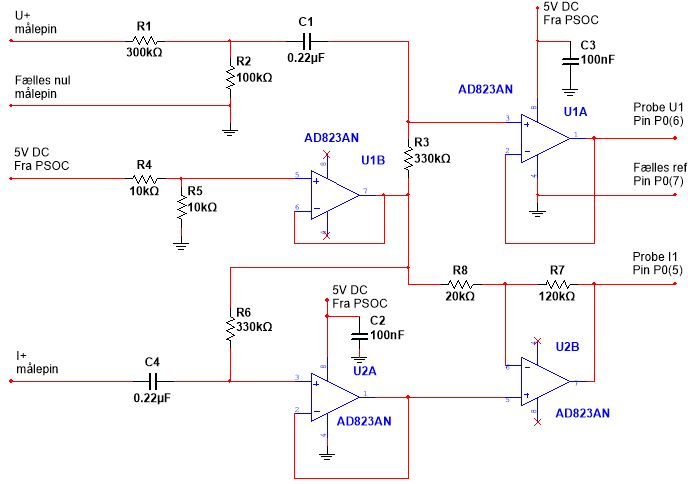
\includegraphics[width=1\textwidth]{figure/MaalHardware}
	\caption{Diagram for hardwaren til Måleenheden}
	\label{fig:MaalHardware}
\end{figure} 

\subsubsection{Spændingsmåling}
Da det er 8V rms, skal det ganges op for at få hele signalet med.
\begin{align}
Vpp = 8V*\sqrt{2} = 11,3Vpp
\end{align}

Den mindste dæmpning der kan laves for at signalerne holder sig inden for 0 - 5V skal derfor være:

\begin{align}
min_{daemp} = \dfrac{11.3}{5} = 2,26 gange
\end{align}

Dette ses realiseret vha. modstand R1 og R2.

\subsubsection{Strømmåling}

Da  den maksimale strøm er 500mA rms vil det give en peak to peak værdi på:

\begin{align}
Ipp = 0,5*\sqrt{2} = 0,71A
\end{align}

Hvilket betyder den maks. må forstærkes med:

\begin{align}
maks_{forstaerkning} = \dfrac{5}{0,71} = 7
\end{align}
Denne forstærkning ses realiseret vha. modstand R7 og R8.  



 